\subsubsection{Progettazione}
\myparagraph{Scopo dell'attività} \label{PS_Progettazione_Scopo}La progettazione ha lo scopo di definire quale sarà l'architettura logica del prodotto, viene svolta dai \textit{Progettisti} prima dell'attività di codifica. Una buona architettura consente di:
\begin{itemize}
	\item Ridurre la complessità del prodotto al fine di facilitare l'attività di codifica;
	\item Organizzare e ripartire le responsabilità di realizzazione;
	\item Realizzare un prodotto garantendo qualità e utilizzando il minor numero di risorse.
\end{itemize} 

\myparagraph{Descrizione della sezione}
La sezione contiene le norme relative all'attività di progettazione che i componenti del gruppo, in particolare i \textit{Progettisti}, devono seguire.

\myparagraph{Aspettative}\label{AspettativeProgettazione}Il gruppo per questa attività si aspetta di definire l'architettura logica del prodotto rispettandone le caratteristiche di qualità. Per assicurare il raggiungimento degli obiettivi di qualità previsti dal \PdQ\ il gruppo intende:
\begin{itemize}
	\item Progettare perseguendo la correttezza per costruzione;
	\item Organizzare e ripartire le responsabilità di realizzazione considerando la natura a \glo{microservizi} del prodotto da realizzare;
	\item Realizzare un prototipo del prodotto, il \glo{\textbf{Proof of Concept}}, che comprenda le funzionalità principali per l'utente della piattaforma;
	\item Documentare quanto progettato attraverso i diagrammi UML;
	\item Progettare il prodotto sfruttando le qualità delle tecnologie da utilizzare;
	\item Progettare il prodotto considerando la facilità di utilizzo dello stesso per l'utente.
\end{itemize}

\myparagraph{Qualità dell'attività di progettazione}\label{QualitàProgettazione}Un'architettura di buona qualità ha come caratteristiche misurabili e osservabili oggettivamente:
\begin{itemize}
	\item \textbf{Sufficienza:} capace di soddisfare tutti i requisiti indicati nell'\AdR; 
	\item \textbf{Comprensibilità:} capace di essere capita da tutti gli stakeholders;
	\item \textbf{Modularità:} suddivisa in parti chiare e ben distinte;
	\item \textbf{Robustezza:} capace di gestire eventi non previsti causati dall'utente e dall'ambiente;
	\item \textbf{Flessibilità:} permette modifiche a costo contenuto al variare dei requisti;
	\item \textbf{Riusabilità:} le sue parti possono essere utilizzate in altre applicazioni;
	\item \textbf{Affidabilità:} svolge quanto previsto;
	\item \textbf{Sicura:} capace di resistere a malfunzionamenti ed evitare possibili intrusioni.
\end{itemize}
Le sue componenti devono essere semplici, coese nel raggiungimento degli obiettivi, incapsulate e con un basso livello di accoppiamento.
I \textit{Progettisti} devono assicurare che l'architettura e le sue componenti presentino le caratteristiche descritte e superino dei test di qualità da loro definiti.

\newpage
\myparagraph{Periodi della progettazione}\label{PeriodiProgettazione}L'attività di progettazione si articola in due parti: 
\paragraph*{Progettazione architetturale} 
Vengono definite le specifiche dell'architettura e delle componenti del prodotto, delle loro interazioni con le restanti parti del sistema e dei test di integrazione. Al termine di questo periodo di progettazione si ottiene la \glo{\textbf{Technology Baseline}} del progetto che conterrà: 
\begin{itemize}
	\item \textbf{Proof of Concept:} primo eseguibile del sistema in grado di dimostrare che la tecnologia selezionata serve in modo efficace allo sviluppo del prodotto atteso;
	\item \textbf{Tecnologie utilizzate:} descrizione dettagliata delle tecnologie impiegate nello sviluppo del progetto, con particolare enfasi sui pregi e i difetti riscontrati;
	\item \textbf{Test di integrazione:} definizione dei test eseguiti per verificare che le varie componenti del sistema, una volta integrate insieme, interagiscano in modo corretto e in conformità con quanto richiesto dai requisiti;
	\item \textbf{Tracciamento delle componenti:} associazione tra requisiti e componenti che li soddisfano.
\end{itemize}

\paragraph*{Progettazione di dettaglio}
Vengono definite le specifiche di dettaglio dell'architettura suddividendo il sistema fino ad arrivare a singole unità ben definite e realizzabili da un singolo programmatore. Al termine di questo periodo di progettazione si ottiene la \glo{\textbf{Product Baseline}} del progetto che conterrà: 
\begin{itemize}
	\item \textbf{Design Pattern:} descrizione dei \glo{design pattern} utilizzati nella definizione dell'architettura, per la soluzione progettuale a problemi ricorrenti riscontrati; ogni design pattern deve essere opportunamente descritto, con una spiegazione del suo significato, ed accompagnato da un diagramma che ne mostri la struttura;
	\item \textbf{Diagrammi UML:} diagrammi realizzati in linguaggio UML versione 2.0, utilizzati per rendere più chiare le soluzioni progettuali adottate; 
	\item \textbf{Test di unità:} definizione dei test eseguiti per verificare che il funzionamento delle varie classi e metodi che implementano il sistema software sia corretto e conforme ai requisiti;
	\item \textbf{Tracciamento delle classi:} associazione tra requisiti e classi che li soddisfano.
\end{itemize}

\myparagraph{Diagrammi UML 2.0}\label{DiagrammiUML}I diagrammi UML sono diagrammi realizzati in linguaggio UML, utilizzati per chiarire le scelte progettuali adottate e ridurre eventuali ambiguità. 
Di seguito vengono analizzati i diagrammi utilizzati.
\paragraph*{Diagrammi delle classi}
Questi diagrammi descrivono il tipo degli oggetti che fanno parte di un sistema.\\
Gli elementi di un diagramma di classe sono:
\begin{itemize}
	\item \textbf{Nome:} nome della classe. Nel caso di un'interfaccia deve essere preceduto dalla direttiva \textbf{$\ll$interface$\gg$};
	\item \textbf{Attributi:} la definizione di un attributo segue il formato:
	\begin{center}
		\textbf{Visibilità nome: tipo [molteplicità] = default [proprietà aggiuntive]}
	\end{center}
	\begin{itemize}
		\item \textbf{Visibilità:} visibilità dell'attributo rispetto ad altre classi, può essere:
		\begin{itemize}
			\item -: visibilità privata;
			\item +: visibilità pubblica;
			\item \#: visibilità protetta;
			\item $\sim$: visibilità di package.
		\end{itemize}
		\item \textbf{Nome:} nome dell'attributo, se l'attributo è costante il nome deve essere scritto in maiuscolo;
		\item \textbf{Tipo:} tipo di dato dell'attributo;
		\item \textbf{Molteplicità:} occorrenze dell'attributo nella classe, il campo è opzionale;
		\item \textbf{Valore di default:} valore predefinito dell'attributo;
		\item \textbf{Proprietà aggiuntive:} eventuali proprietà ritenute importanti, il campo è opzionale.
	\end{itemize}
	\item \textbf{Operazioni:} rappresentano le azioni eseguibili dalla classe, la definizione di una operazione segue il formato:
	\begin{center}
		\textbf{Visibilità nome [lista-parametri] : tipo-ritorno [proprietà aggiuntive]}
	\end{center}
	\begin{itemize}
		\item \textbf{Visibilità:} visibilità dell'operazione rispetto ad altre classi indicata come per gli attributi;
		\item \textbf{Nome:} nome dell'operazione;
		\item \textbf{Lista-parametri:} lista dei parametri dell'operazione;
		\item \textbf{Return-type:} tipo di ritorno dell'operazione;
		\item \textbf{Proprietà aggiuntive:} eventuali proprietà ritenute importanti, il campo è opzionale.
	\end{itemize}
\end{itemize} 
I diagrammi delle classi sono collegati tra loro tramite \textbf{relazioni di dipendenza}, la modifica di un elemento di un diagramma può cambiarne la definizione di un altro.
Le relazioni di dipendenza previste sono:
	\begin{itemize}
		\item \textbf{Dipendenza:} gli oggetti di una classe A utilizzano brevemente gli oggetti di un'altra classe B, l'associazione esiste per un tempo limitato;
		\begin{center}
			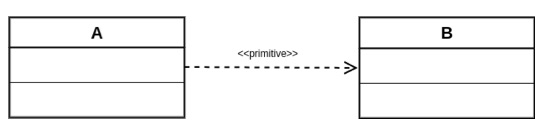
\includegraphics[scale=0.4]{Immagini/UML/Dipendenza} \\
			\captionof{figure}{Dipendenza fra classi}
		\end{center}
		\item \textbf{Associazione:} la classe A contiene dei campi dati o delle istanze di un'altra classe B. \\ Le molteplicità possibili sono:
		\begin{itemize}
			\item \textbf{1:} A possiede un'istanza di B;
			\item \textbf{0..1:} A possiede 0 o 1 istanze di B;
			\item \textbf{0..*:} A possiede 0 o più istanze di B;
			\item \textbf{*:} A possiede più istanze di B.
		\end{itemize}
		\begin{center}
			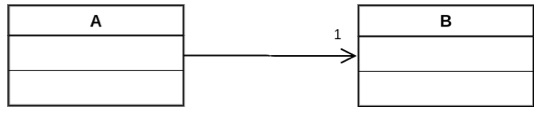
\includegraphics[scale=0.4]{Immagini/UML/Associazione} \\
			\captionof{figure}{Associazione fra classi}
		\end{center}
		\item \textbf{Aggregazione:} la classe A possiede un riferimento ad un oggetto di un'altra classe B che può essere condiviso, l'aggregato B non ha senso di esistere senza l'aggregante A;
		\begin{center}
			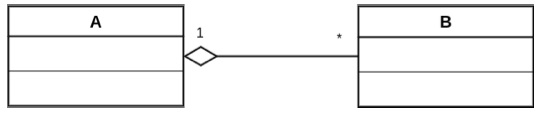
\includegraphics[scale=0.4]{Immagini/UML/Aggregazione}\\
			\captionof{figure}{Aggregazione fra classi}
		\end{center}
		\item \textbf{Composizione:} la classe A possiede un oggetto di un'altra classe B, solo l'oggetto intero può creare e distruggere le sue parti;
		\begin{center}
			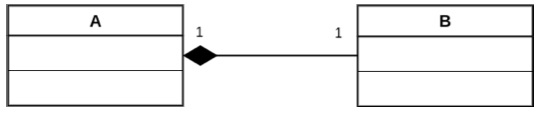
\includegraphics[scale=0.4]{Immagini/UML/Composizione} \\
			\captionof{figure}{Composizione fra classi}
		\end{center}
		\item \textbf{Generalizzazione:} la classe A generalizza un'altra classe B se ogni oggetto di B è anche un oggetto di A;
		\item \textbf{Subtyping:}  la classe A implementa l'interfaccia B. 
		\begin{center}
				\begin{minipage}{0.4\textwidth}
					\begin{center}
						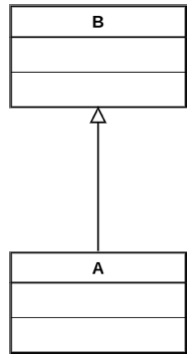
\includegraphics[scale=0.4]{Immagini/UML/Generalizzazione}\\
						\captionof{figure}{Generalizzazione fra classi}
					\end{center}
			\end{minipage}
			\begin{minipage}{0.5\textwidth}
				\begin{center}
						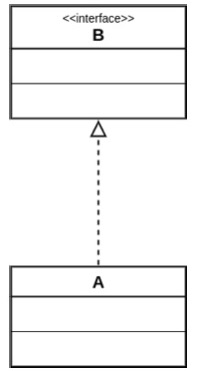
\includegraphics[scale=0.385]{Immagini/UML/Subtyping}\\
					\captionof{figure}{Subtyping fra classi}
				\end{center}
			\end{minipage}
		\end{center}	
	\end{itemize}

\paragraph*{Diagrammi dei package}
Un package rappresenta un raggruppamento di un numero arbitrario di elementi UML in una unità di livello più alto, può quindi contenere classi (anche astratte), un altro package e interfacce. Ogni elemento di un package, identificativo di un \glo{namespace}, può avere visibilità pubblica(+) o privata(-) e deve avere un nome completamente qualificato secondo lo schema: 
\begin{center}
	\textbf{package::package::...::classe}
\end{center}
I diagrammi dei package documentano le dipendenze tra le classi che dovrebbero seguire tutte la stessa direzione evitando le dipendenze circolari.

\paragraph*{Diagrammi delle attività}
Questi diagrammi descrivono la logica procedurale e i processi di business, aiutando a descrivere gli aspetti dinamici dei casi d'uso.\\
Gli elementi di un diagramma di attività sono:
\begin{itemize}
	\item \textbf{Token:} vengono prodotti e consumati durante l'esecuzione;
	\item \textbf{Nodo iniziale:} rappresenta il punto d'inizio dell'esecuzione dell'attività, genera token;
	\item \textbf{Nodo di fine flusso:} rappresenta un punto di terminazione di un percorso di esecuzione, l'attività può continuare su altri percorsi;
	\item \textbf{Nodo finale:} rappresenta il punto di terminazione dell'esecuzione dell'attività, consuma token;
	\begin{center}
		\begin{minipage}{0.3\textwidth}
			\centering
			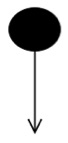
\includegraphics[scale=0.2]{Immagini/UML/NodoIniziale}
			\captionof{figure}{Nodo iniziale}
		\end{minipage}
		\begin{minipage}{0.3\textwidth}
			\centering
			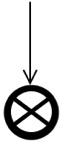
\includegraphics[scale=0.2]{Immagini/UML/NodoFineFlusso}
			\captionof{figure}{Nodo fine flusso}
		\end{minipage}
		\begin{minipage}{0.3\textwidth}
			\centering
			
\includegraphics[scale=0.19]{Immagini/UML/NodoFinale}
			\captionof{figure}{Nodo finale}
		\end{minipage}
	\end{center}
	\item \textbf{Activity:} rappresenta un'azione all'interno dell'attività, identificata da una breve descrizione;
	\item \textbf{Subactivity:} rappresenta una sotto-attività utilizzata per descrivere un'azione che ne comprende altre al suo interno, il suo diagramma viene fornito separatamente. Ogni sotto-attività è composta dall'input, dall'output e dalle azioni contenute.
	\begin{center}
		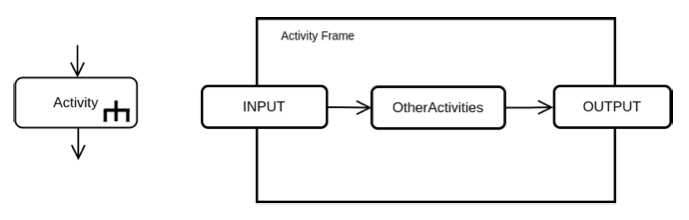
\includegraphics[scale=0.4]{Immagini/UML/Sottoattivita}
		\captionof{figure}{Attività che presenta una sotto-attività}
	\end{center}
	\item \textbf{Pin:} rappresenta un parametro prodotto o consumato da un'azione, va indicato il formato del parametro;
	\begin{center}
		\centering
		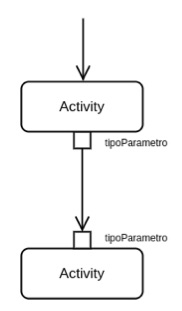
\includegraphics[scale=0.4]{Immagini/UML/Pin}
		\captionof{figure}{Attività che presenta un pin}
	\end{center}
	\item \textbf{Fork:} rappresenta un punto d'inizio di un'elaborazione parallela all'interno dell'attività, produce un token per ogni processo;
	\item \textbf{Join:} rappresenta un punto di sincronizzazione tra i processi paralleli, consuma i token in ingresso e ne genera solo uno;
	\item \textbf{Branch:} rappresenta un punto di decisione tra i possibili percorsi di esecuzione in base alla guardia associata;
	\item \textbf{Merge:} rappresenta un punto di unione dei diversi percorsi di esecuzione (non paralleli) generati in seguito ad un branch, il token viene solo instradato;
	\begin{center}
		\begin{minipage}{0.4\textwidth}
			\centering
			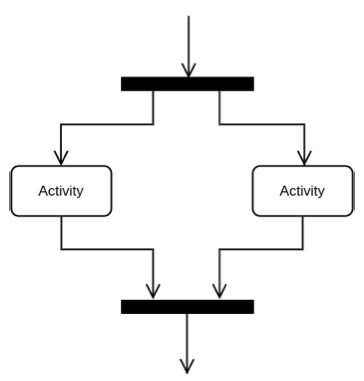
\includegraphics[scale=0.453]{Immagini/UML/ForkJoin}
			\captionof{figure}{Fork e Join}
		\end{minipage}
		\begin{minipage}{0.4\textwidth}
			\centering
			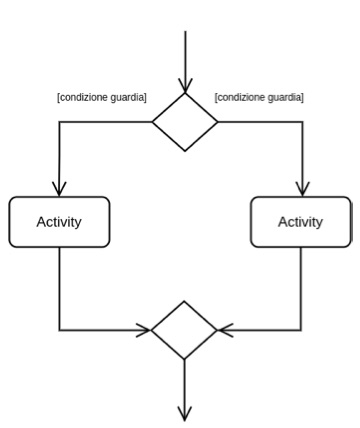
\includegraphics[scale=0.4]{Immagini/UML/BranchMerge}
			\captionof{figure}{Branch e Merge}
		\end{minipage}
	\end{center}
	\item \textbf{Segnale:} rappresenta un evento esterno, generato in modo non bloccante e catturato in modo bloccante, all'interno dell'attività;
	\begin{center}
		\centering
		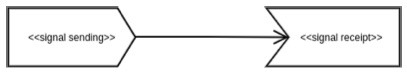
\includegraphics[scale=0.5]{Immagini/UML/Segnali}
		\captionof{figure}{Segnali in un diagramma attività}
	\end{center}
	\item \textbf{Timeout:} rappresenta un'attesa bloccante all'interno dell'attività, di cui deve essere specificata la durata e l'unità di misura, o un evento ripetuto nel tempo;
	\begin{center}
		\centering
		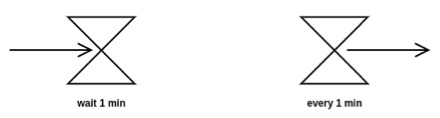
\includegraphics[scale=0.5]{Immagini/UML/Timeout}
		\captionof{figure}{Timeout in un diagramma attività}
\end{center}
	\item \textbf{Swimlane:} fornisce una responsabilità all'esecuzione delle azioni all'interno di un'attività.
\end{itemize}

\paragraph*{Diagrammi di sequenza}
I diagrammi di sequenza descrivono la collaborazione di un gruppo di oggetti che devono implementare collettivamente un comportamento.
Gli elementi utilizzati in questi diagrammi sono i seguenti:
\begin{itemize}
	\item \textbf{Partecipante:} entità che detiene il flusso di esecuzione del caso d'uso, è composto di due parti:
	\begin{itemize}
		\item \textbf{Nome:} nome dell'entità partecipante;
		\item \textbf{Barra di attivazione:} indica il periodo di tempo durante il quale il partecipante è attivo;
	\end{itemize}
	\item \textbf{Messaggio:} rappresenta dati e operazioni scambiati tra partecipanti, può essere di una delle seguenti tipologie:
	\begin{itemize}
		\item \textbf{Sincrono:} il chiamante rimane in attesa della risposta;
		\item \glo{\textbf{Asincrono:}} il chiamante non attende la risposta; 
		\item \textbf{Ritorno:} messaggio di ritorno riferito ad un precedente messaggio di chiamata;
		\item \textbf{Creazione:} messaggio di creazione di un nuovo partecipante da parte del partecipante chiamante;
		\item \textbf{Distruzione:} messaggio di distruzione di un partecipante da parte del partecipante chiamante.
	\end{itemize}
\end{itemize}
\begin{center}
	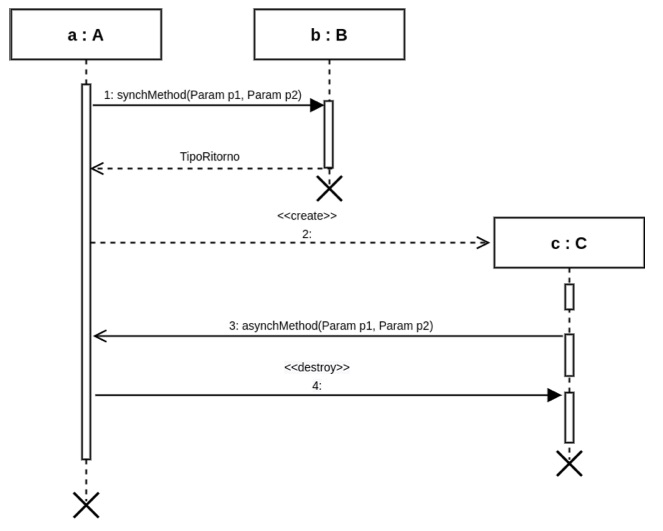
\includegraphics[scale=0.5]{Immagini/UML/DSequenza} \\
	\captionof{figure}{Esempio di diagramma di sequenza}
\end{center}

\paragraph*{Diagrammi dei casi d'uso}
Un caso d'uso è un'insieme di scenari (sequenze di azioni) che hanno in comune uno scopo finale per un utente. I diagrammi dei casi d'uso sono una rappresentazione grafica dei casi d'uso analizzati nel documento di \AdR{}. Vengono messi in evidenza:
\begin{itemize}
	\item \textbf{Attori:} rappresentano tutto ciò che è esterno al sistema e interagisce con esso;
	\item \textbf{Use Case:} rappresentano le attività associate al sistema.
\end{itemize}
Le eventuali relazioni tra gli use case del sistema rappresentate in questi diagrammi sono: 
\begin{itemize}
	\item \textbf{Inclusione:} si ha quando vi sono funzionalità comuni fra più casi d'uso, lo use case B è incondizionatamente incluso nell'esecuzione dello use case A;
	\begin{center}
		\centering
		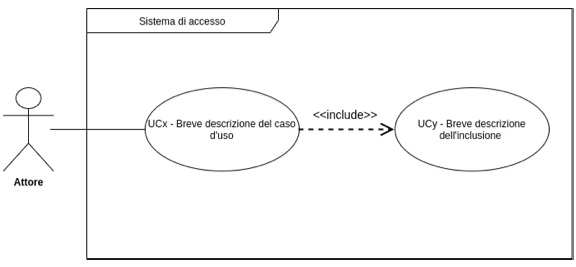
\includegraphics[scale=0.4]{Immagini/UML/Inclusione}
		\captionof{figure}{Inclusione casi d'uso}
	\end{center}
	\item \textbf{Estensione:} si ha se ogni istanza dello use case A esegue lo use case B in modo condizionato, l'esecuzione di B interrompe A;
	\begin{center}
		\centering
		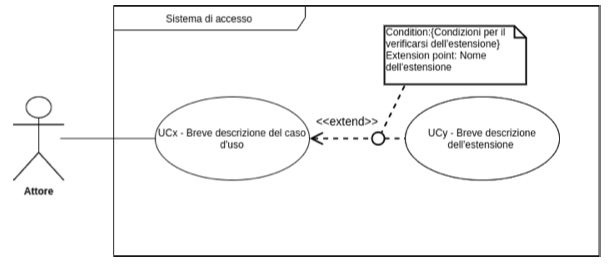
\includegraphics[scale=0.4]{Immagini/UML/Estensione}
		\captionof{figure}{Estensione casi d'uso}
	\end{center}
	\item \textbf{Generalizzazione:} si ha quando si vogliono aggiungere o modificare caratteristiche base, in particolare si ha che:
	\begin{itemize}
		\item L'attore A è generalizzazione dell'attore B se B condivide almeno le funzionalità di A;
		\item I casi d'uso figli aggiungono funzionalità rispetto ai padri o ne modificano il comportamento.
	\end{itemize}
	\begin{center}
		\begin{minipage}{0.4\textwidth}
			\centering
			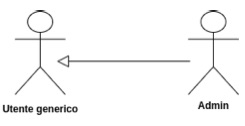
\includegraphics[scale=0.4]{Immagini/UML/GeneralizzazioneAttori}
			\captionof{figure}{Generalizzazione tra attori}
		\end{minipage}
		\begin{minipage}{0.5\textwidth}
			\centering
			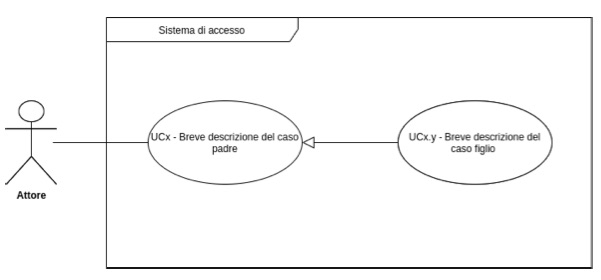
\includegraphics[scale=0.4]{Immagini/UML/GeneralizzazioneUC}
			\captionof{figure}{Generalizzazione Casi d'uso}
	\end{minipage}
	\end{center}
\end{itemize} 

\myparagraph{Metriche}\label{MProgettazione}Di seguito vengono presentate le metriche utilizzate per garantire il controllo sulla qualità. Per una descrizione sullo standard di riferimento e un elenco completo di tutte le metriche applicate si rimanda alla sezione \S\ref{9126} dell'appendice. 
\begin{itemize}
	\item \textbf{MPDS03: Tempo di caricamento delle schermate;}\hypertarget{MCViste}\\
	Il valore stabilisce la velocità con cui le varie schermate del prodotto software vengono caricate e mostrate all'utente, viene calcolato attraverso uno strumento automatico;
	\item \textbf{MPDS04: Facilità di utilizzo;}\hypertarget{MFUtilizzo}\\
	Il valore stabilisce la semplicità per un utente di raggiungere quanto cercato valutando il numero di click medio per raggiungere il contenuto desiderato;
	\item\textbf{MPDS05: Facilità di apprendimento}\hypertarget{MFApprendimento}\\
	Il valore stabilisce la semplicità per un utente di raggiungere quanto cercato all'interno del sito calcolando la media dei minuti necessari per raggiungere le pagine ricercate;
	\item\textbf{MPDS06:  Profondità della gerarchia}\hypertarget{MPGerarchia}\\
	Il valore risultante viene calcolato individuando la profondità della gerarchia delle schermate rispetto alla principale.
\end{itemize}